\chapter{Experimental work and Result} % Main chapter title
\label{Chapter3} % Change X to a consecutive number; for referencing this chapter elsewhere, use \ref{ChapterX}


%----------------------------------------------------------------------------------------
%	SECTION 1
%----------------------------------------------------------------------------------------
\section{Experimental Setup}


%----------------------------------------------------------------------------------------
%	SUBSECTION 1
%----------------------------------------------------------------------------------------
\subsection{Camera and MatchID Setup}

An Allied Vision Manta 505B 2/3'' camera coupled to an Opto Engineering TC 23 36 telecentric lens were used for image formation and acquisition. The camera is equipped with Charge-Coupled Device (CCD) sensor with pixel resolution of 2452 (H) $\times$ 2056 (V) (5MP) and sensor size of 2/3''. The monovision camera-lense optical system was fixed on a tripod and its spatial position oriented with regard to the target surface of interest. The telecentric lens has a magnification factor of \num{0.243}$\times$, allowed to image a field of view, in the object space, of 36.2$\times$27.1 \si{\milli\meter\squared}. The front of the lens was positioned at a working distance of 103.5 \si{\milli\meter} with an aperture of $f$/8, yielding a field of depth of 11 \si{\milli\meter}.

A high power adjustable ring light was used to illuminate the region of interest. A monochromatic version corresponding to a green wavelength of \num{525} \si{\nano\meter} was used from which the highest spectral response of the camera sensor will be expected.

All the specimens were painted to obtain a speckle pattern suitable for image correlation. A thin layer of white paint was firstly added using a mate spray, followed by a diffuse distribution of black paint to create a unique local pattern across the region of interest at the crack tip (Figure~\ref{fig:Fig17}).

\begin{figure}[t]
	\centering
	\includegraphics[width=.9\textwidth]{Figures/SpecklePattern}
	\decoRule
	\caption{(a) Speckle pattern typically obtained for DIC measurements (2452 $\times$ 2056
		pixels\textsuperscript{2}); (b) Histogram
		of the
		speckle image
		(256
		gray levels, 8 bits camera).}
	\label{fig:Fig17}
\end{figure}

%\section{DIC measurements and settings}

The DIC setting parameters can have a significant influence on the kinematic fields obtained by image correlation (\textit{e.g.} subset size, subset step, \ldots) and numerical differentiation (\textit{e.g.} strain windows size) algorithms \cite{Pereira2018566}. These settings represent fundamental parameters since they will define the spatial resolution and accuracy associated to the DIC measurements, both in displacement and strain fields.  Therefore, a parametric study was carried out to justify the DIC setting for the current
application, in a balance between resolution and spatial resolution. This study was carried ot in the Parametric Module of MatchID 2D software.
\begin{table}[]
	\centering
	\begin{tabular}{c c}
		\hline
		Correlation   Coefficient: & ZNSSD \\ 
		Interpolation order: & Bicubic Splines \\ 
		Transformation order: & Affine \\
		Subset size: & 21 \\
		Step size: & 5 \\
		Maximum rigid body estimation: & 100 \\ 
		Strain Estimation(\%): & 5 \\ 
		Precision: & 0.001 \\ 
		Maximum iterations: & 20 \\ 
		Noise handling: & Gaussian \\ 
		Kernel Size: & 5 \\ 
		History: & Spatial \\ 
		Strainwindow size: & 7 \\ 
		Tolerance on number of points: & 0 \\ 
		Strain interpolation: & Q4 \\ 
		Strain Convention: & Green-Lagrange \\ \hline
	\end{tabular}
	\caption{MatchID parameters used}
	\label{tab:MatchID_param}
\end{table}
\ref{tab:MatchID_param} defines the range of values defined in this performance analysis which includes the subset size ($f_s$), subset step, affine and quadratic displacement shape functions, the strain windows size and the order of the polynomial fitting function. The pre-selected range of values are deemed to be representative of the range of acceptable DIC setting parameters. For instance, The lower pixel boundary is constrained by aliasing effects, which is a function of the speckle size on the imaged pattern. The subset size defines the target matching pattern used in the correlation algorithm. A rule of thumb will be three contrasted speckles per subset. The average speckle size was determined as 4.5 pixels. Therefore, the minimum subset step was set to 15 pixels. The upper pixel limit can be problem-dependent, taking into account the deformation gradients expected within the region of interest, in a balance between spatial resolution and resolution. As a guideline, larger subsets improves the resolution but decreases spatial resolution. Parameters such as the subset step ($f_p$) (distance between centroids of adjacent subsets, units: pixels) and the strain window $\varepsilon_w$ (number of subsets central points used to define a mesh of data points over which a piecewise polynomial fitting will be applied, using least-square regression, for strain reconstruction) will define a strain spatial resolution ($\Delta \varepsilon$) and virtual strain gauge (VSG), respectively, according to the following relationships \cite{Lava2013576,Pereira2018566}: $\Delta \varepsilon = (\varepsilon_w-1)f_p + f_s$ and $\mbox{VSG} = (\varepsilon_w-1)f_p + 1$ (unit: pixel). For convenience, these parameters can be converted to physical units in the object space (\textit{e.g.} mm), by simple multiplication by the conversion factor of the optical imaging system. All these external DIC parameters, therefore, must be carefully selected in the current study.


A single pair of images, including a reference and deformed image at a force of about 100 N were selected to carry out this study. The obtained results are shown in Figure ?. In this plot the signal of interest, is plotted with regard to a measure of the strain spatial resolution given by the parameter Virtual Strain Gauge (VSG). Both the $y$ component of the displacement and $\varepsilon_{yy}$ component of strain are presented to support the DIC setting selection. Therefore
%----------------------------------------------------------------------------------------
%	SUBSECTION 2
%----------------------------------------------------------------------------------------
\subsection{Servohydraulic test machine and grips Setup}

The servohydraulic test machine, was setup by Mr Martins. The first step was to assembled the grips in the press. They are screwed, for the first one, into one static part of the press, the upper side. The other grip is placed in the moving part. Between every test, the grips must be disassembled and well screwed to maintain each specimen, as well as possible. To change the specimen between two tests, manual command are used to elevate the moving part of the press and avoid the tension in the grips. Of course this pre-tension was also applied on the specimen before the beginning of the test, in order to avoid specimen movement due to the screwed grips.
Then a velocity of 0.033\si{\milli\meter\per\second} mm/s was defined in the controller of the servohydraulic test machine. A 10\si{\kilo\newton} load was also input to be sure that the displacement will occur correctly. Afterwards a velocity of 0.015\si{\milli\meter\per\second} was finally applied. The position and the load are given at each time by the MTS software controller. Moreover, a plot is created in real time.

\begin{figure}[t]
	\centering
	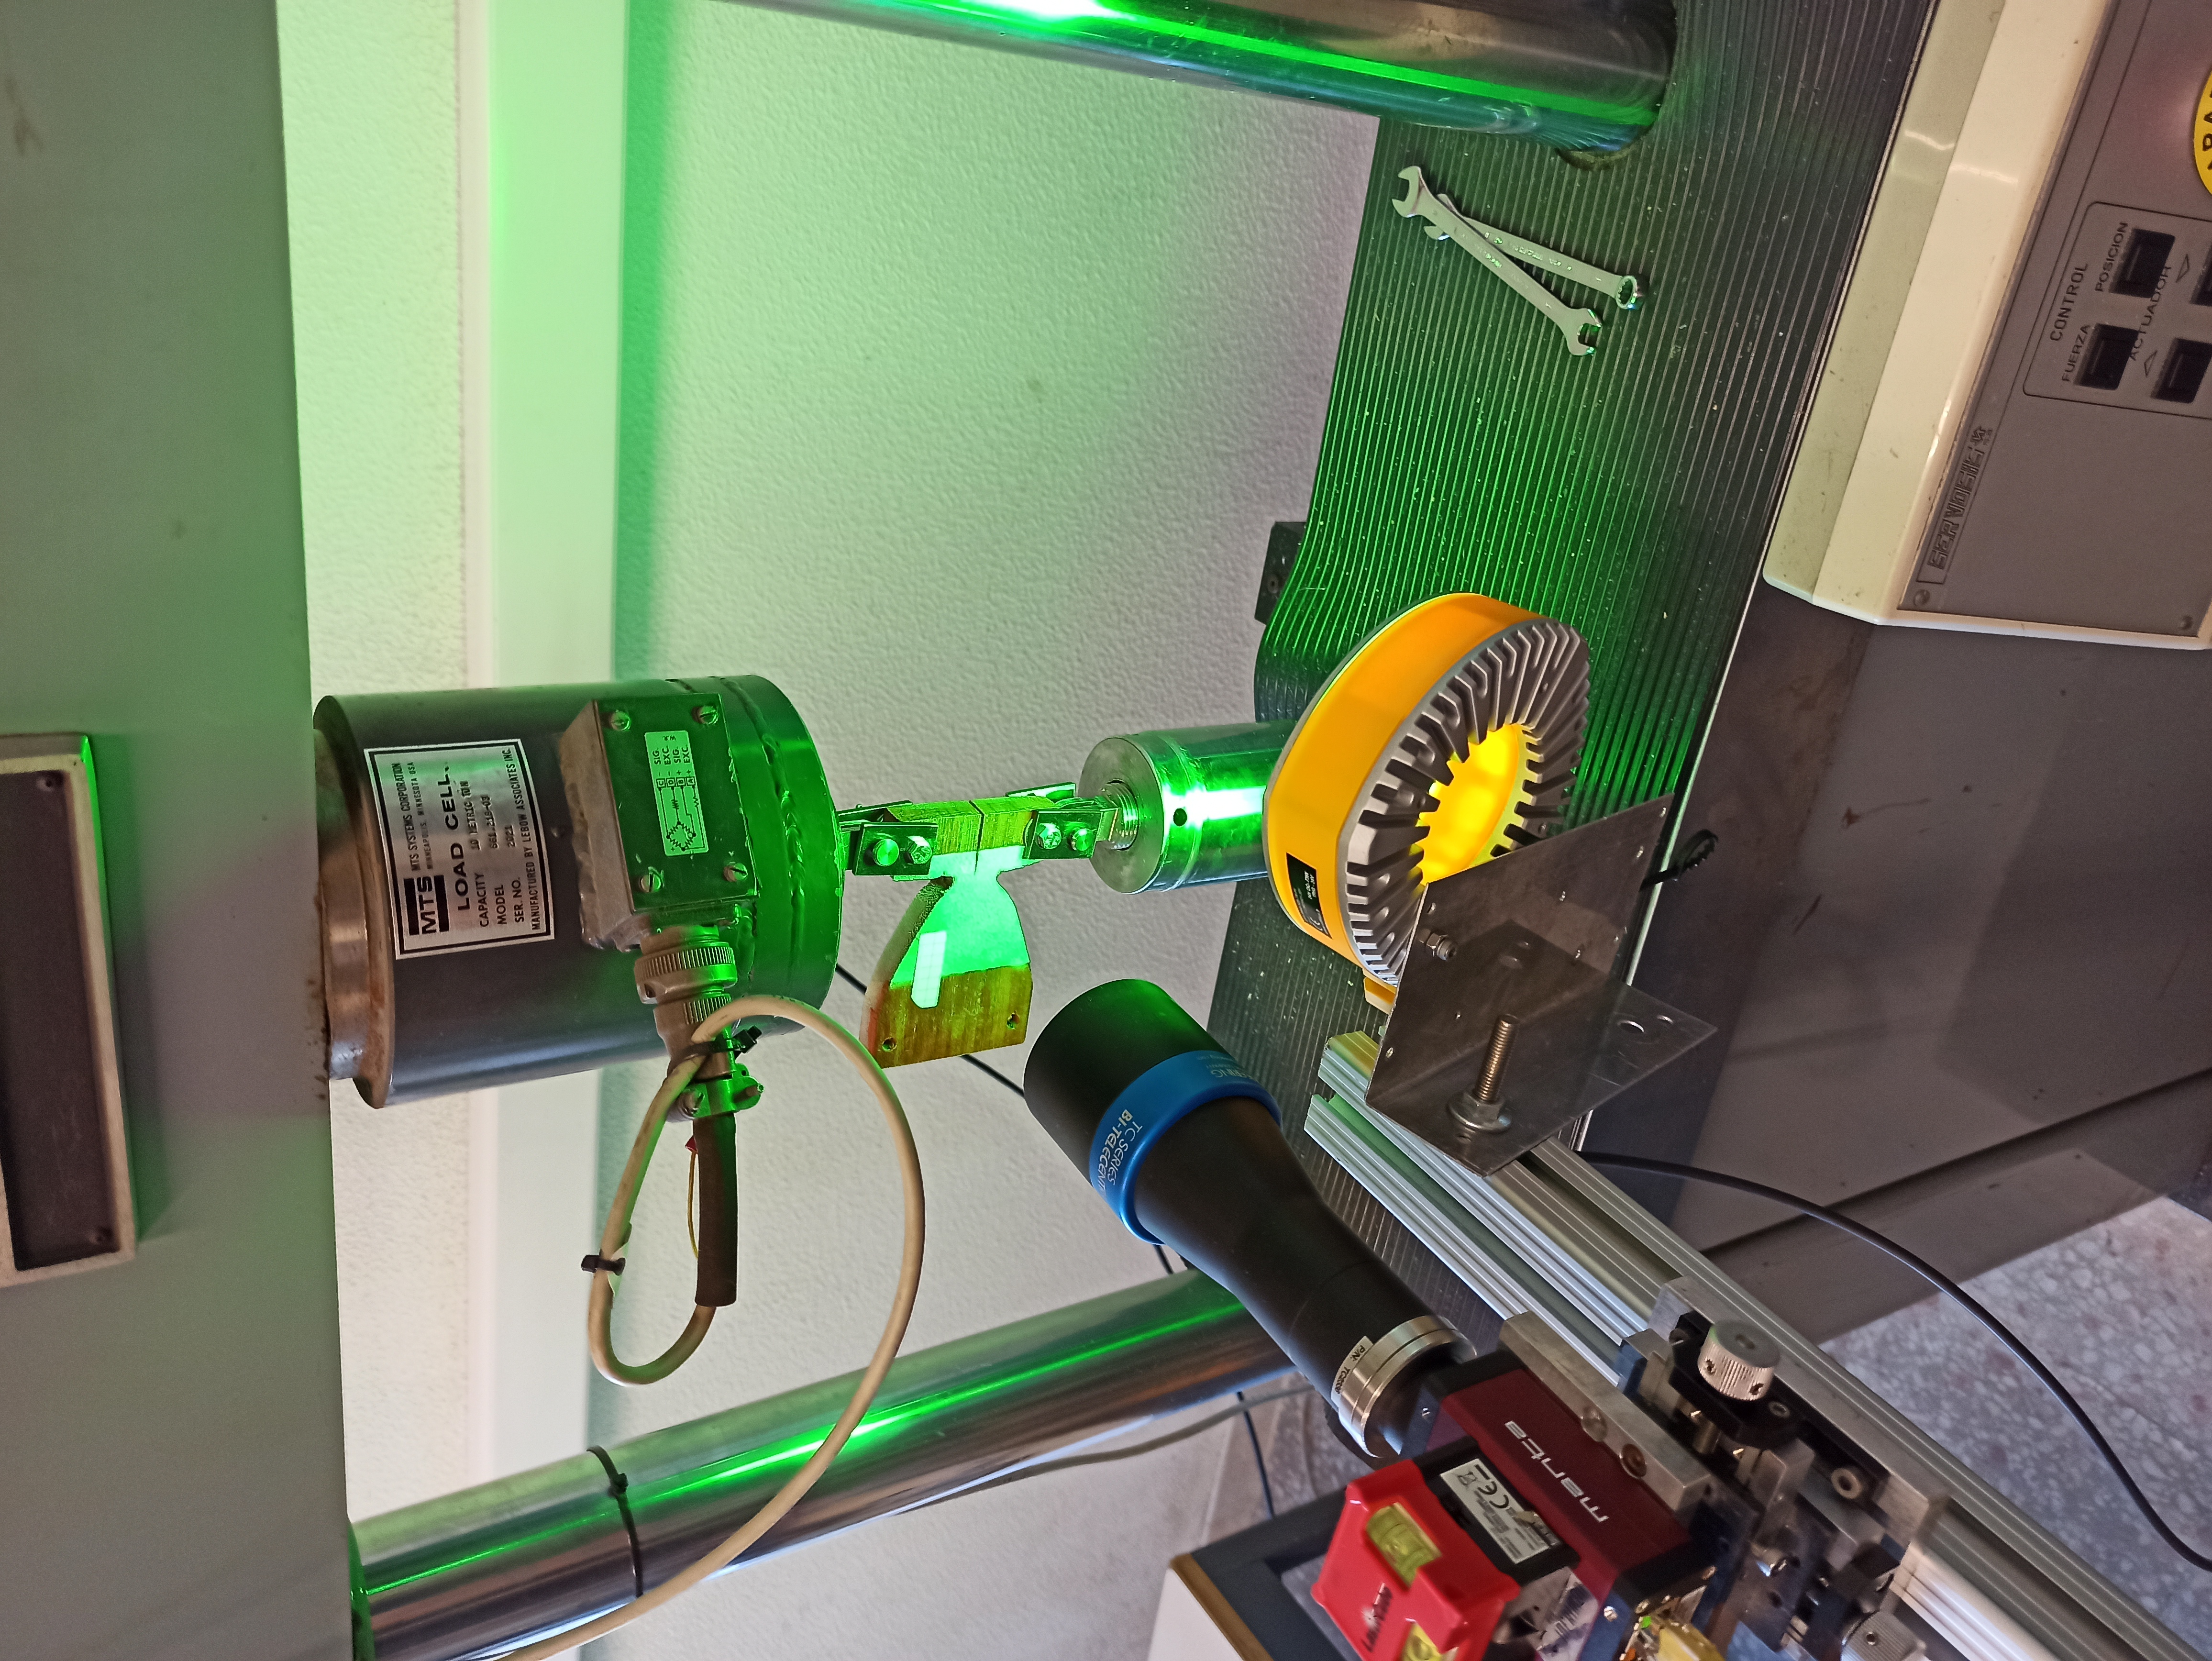
\includegraphics[scale=0.05,angle=-90]{Figures/SetUp}
	\decoRule
	\caption[Final setup]{Setup composed of the camera and it lens linked to MatchId, the green constant light, tripods, the hydraulic press and the specimen griped to it.}
	\label{fig:Fig18}
\end{figure}

The temperature and relative humidity during the test were controlled thanks to a sensor placed in the test room. The \ref{fig:Fig19} gives an idea of the conditions which were almost constant, even if the temperature increase with the rise of the servohydraulic test machine utilization time.

\begin{figure}[t]
	\centering
	\includegraphics[scale=0.08]{Figures/Temperature_ relative_humidity}
	\decoRule
	\caption[Climatic conditions of the test]{Climatic conditions of the test in a closed room}
	\label{fig:Fig19}
\end{figure}

%----------------------------------------------------------------------------------------
%	SUBSECTION 3
%----------------------------------------------------------------------------------------
\subsection{MMCG specimen last preparation and Moisture Content reach}
To test the specimens at the weighted MC, plots as the \ref{fig:Fig15_a} were used. Indeed, by looking to their weight when they were out of the water, a MC was obtained, and by looking to the difference between the current MC and the weighted one can be given in terms of hours. So it was possible to have an approximation of the time before doing the experiments.

All the specimens were painted to obtain a pattern which allows a treatment of the images as explained before. Indeeed it will be necessary for MatchID to have speckles composed of a given number of pixels. A white first layer was added and a black point cloud was a second painting layer. All the paint used, are mate ones, and not brilliant ones. The dimension of the painted areas are not precisely defined. It is not necessary to paint the heels, because they were not studied. But even some painted zone are not really interesting as the extremity of MMCG specimen shapes. 
\begin{figure}[th]
	\centering
	\includegraphics[scale=0.08]{Figures/Painted_specimen}
	\caption[Padouck painted specimen]{Padouck painted specimen before experimental test}
	\label{fig:paintedSpec}
\end{figure}
As it is presented on \ref{fig:paintedSpec} the characteristic pattern replace the grid from the grid method as used in \parencite{Reference7} or a markers tracking method like in \parencite{Reference18} work. The pattern is different for every specimen. From the second sample tested, a scale was added to the specimens. But finally this scale was not useful. Indeed, DIC images allow to fix some dimensions and measured others.
The precrack was measured again and more precisely with a caliper. The measure can change, due to the swelling of the wet specimens.

Dimensions as the crack length or the thickness of the specimens were measured again due to their evolution because of the swelling process. For some of the specimens, the grips were embedded in advance to remove some material which could distort the final weight. Then they are weighted a last time. The table \ref{tab:LastMC} presents the MC reached by all the specimens when there were tested.
\newpage
\begin{table}[th]
	\centering
	\begin{tabular}{cccc}
				
		\multicolumn{1}{c}{Name of   the specimen} & \multicolumn{1}{c}{dry Weight {[}g{]}} & \multicolumn{1}{c}{Tested weight} & \multicolumn{1}{c}{MC} \\ 
		\multicolumn{4}{c}{} \\ 
		\multicolumn{4}{c}{\cellcolor[HTML]{F4B084}room t° \& room MC} \\ 
		\multicolumn{1}{c}{E1O1} & \multicolumn{1}{c}{39,446} & \multicolumn{1}{c}{42,395} & \multicolumn{1}{c}{7,48\%} \\ 
		\multicolumn{1}{c}{E1O2} & \multicolumn{1}{c}{36,223} & \multicolumn{1}{c}{38,9057} & \multicolumn{1}{c}{7,41\%} \\ 
		\multicolumn{1}{c}{E1O3} & \multicolumn{1}{c}{35,496} & \multicolumn{1}{c}{38,108} & \multicolumn{1}{c}{7,36\%} \\ 
		\multicolumn{1}{c}{E1P1} & \multicolumn{1}{c}{52,243} & \multicolumn{1}{c}{54,867} & \multicolumn{1}{c}{5,02\%} \\ 
		\multicolumn{1}{c}{E1P2} & \multicolumn{1}{c}{61,411} & \multicolumn{1}{c}{64,652} & \multicolumn{1}{c}{5,28\%} \\ 
		\multicolumn{1}{c}{E1P3} & \multicolumn{1}{c}{61,493} & \multicolumn{1}{c}{64,507} & \multicolumn{1}{c}{4,90\%} \\ 
		\multicolumn{1}{c}{E1I1} & \multicolumn{1}{c}{51,67} & \multicolumn{1}{c}{54,858} & \multicolumn{1}{c}{6,17\%} \\ 
		\multicolumn{4}{c}{\cellcolor[HTML]{F4B084}room t° \& MC$\sim$30\%} \\ 
		\multicolumn{1}{c}{E2O1} & \multicolumn{1}{c}{34,219} & \multicolumn{1}{c}{40,914} & \multicolumn{1}{c}{19,57\%} \\ 
		\multicolumn{1}{c}{E2O2} & \multicolumn{1}{c}{35,511} & \multicolumn{1}{c}{41,601} & \multicolumn{1}{c}{17,15\%} \\ 
		\multicolumn{1}{c}{E2O3} & \multicolumn{1}{c}{36,862} & \multicolumn{1}{c}{43,8} & \multicolumn{1}{c}{18,82\%} \\ 
		\multicolumn{1}{c}{E2P1} & \multicolumn{1}{c}{63,15} & \multicolumn{1}{c}{72,273} & \multicolumn{1}{c}{14,45\%} \\ 
		\multicolumn{1}{c}{E2P2} & \multicolumn{1}{c}{64,803} & \multicolumn{1}{c}{74,965} & \multicolumn{1}{c}{15,68\%} \\ 
		\multicolumn{1}{c}{E2P3} & \multicolumn{1}{c}{63,154} & \multicolumn{1}{c}{71,832} & \multicolumn{1}{c}{13,74\%} \\ 
		\multicolumn{4}{c}{\cellcolor[HTML]{F4B084}room t° \& MC$\sim$20\%} \\ 
		\multicolumn{1}{c}{E3O1} & \multicolumn{1}{c}{37,436} & \multicolumn{1}{c}{46,485} & \multicolumn{1}{c}{24,17\%} \\ 
		\multicolumn{1}{c}{E3O2} & \multicolumn{1}{c}{32,745} & \multicolumn{1}{c}{41,772} & \multicolumn{1}{c}{27,57\%} \\ 
		\multicolumn{1}{c}{E3O3} & \multicolumn{1}{c}{36,449} & \multicolumn{1}{c}{46,434} & \multicolumn{1}{c}{27,39\%} \\ 
		\multicolumn{1}{c}{E3P1} & \multicolumn{1}{c}{64,831} & \multicolumn{1}{c}{76,897} & \multicolumn{1}{c}{18,61\%} \\ 
		\multicolumn{1}{c}{E3P2} & \multicolumn{1}{c}{65,323} & \multicolumn{1}{c}{77,427} & \multicolumn{1}{c}{18,53\%} \\ 
		\multicolumn{1}{c}{E3P3} & \multicolumn{1}{c}{60,43} & \multicolumn{1}{c}{74,757} & \multicolumn{1}{c}{23,71\%} \\ 
		\multicolumn{4}{c}{\cellcolor[HTML]{F4B084}fridge samples} \\ 
		\multicolumn{1}{c}{E4O1} & \multicolumn{1}{c}{40,233} & \multicolumn{1}{c}{52,592} & \multicolumn{1}{c}{30,72\%} \\ 
		\multicolumn{1}{c}{E4P1} & \multicolumn{1}{c}{57,116} & \multicolumn{1}{c}{64,696} & \multicolumn{1}{c}{13,27\%} \\ 
		\multicolumn{1}{c}{E4I1} & \multicolumn{1}{c}{46,467} & \multicolumn{1}{c}{67,599} & \multicolumn{1}{c}{45,48\%} \\ 
		\multicolumn{4}{c}{\cellcolor[HTML]{F4B084}oven sample} \\ 
		\multicolumn{1}{c}{E5O1} & \multicolumn{1}{c}{38,104} & \multicolumn{1}{c}{40,172} & \multicolumn{1}{c}{5,43\%} \\ 
		\multicolumn{1}{c}{E5P1} & \multicolumn{1}{c}{59,767} & \multicolumn{1}{c}{66,339} & \multicolumn{1}{c}{11,00\%} \\ 
		\multicolumn{1}{c}{E5I1} & \multicolumn{1}{c}{51,828} & \multicolumn{1}{c}{66,718} & \multicolumn{1}{c}{28,73\%} \\ 
		\multicolumn{4}{c}{\cellcolor[HTML]{F4B084}resting samples} \\ 
		\multicolumn{1}{c}{Pbis} & \multicolumn{1}{c}{64,574} & \multicolumn{1}{c}{67,301} & \multicolumn{1}{c}{4,22\%} \\ 
		\multicolumn{1}{c}{Pter} & \multicolumn{1}{c}{60,379} & \multicolumn{1}{c}{63,418} & \multicolumn{1}{c}{5,03\%} \\ \hline
	\end{tabular}
	\caption{Moisture Content in every tested samples}
	\label{tab:LastMC}
\end{table}
\newpage
%----------------------------------------------------------------------------------------
%	SUBSECTION 4
%----------------------------------------------------------------------------------------
\subsection{Difficulties and issues}

One of the main problem results of MMCG shapes and the small distance between holes and specimen extremities. It involves several cracks in the heel between the hole and the extremity of the sample. It prevents the observation and analysis of the fracture. This solution which was induced by previous work as \parencite{Reference7} is the use of washers. Indeed, by applying a compressive tension on each side of the specimen, it reduces the stress applied on the holes and it distributes the load in a wider area (the washers surface). \parencite{Reference7} have glued this washer in previous work. In this one it was chosen to strength screw the nut to increase the compressive load created by the washers. Without torque wrench, it is difficult to give an average of the washers constraint exerted. But then this tool was find and used. An approximation of the couple needed to screw and avoid the crack in the hole area is 6.9\si{\newton\per\meter}. By using the \ref{eq:Washers compressive load} formula below, an average is given. Indeed, the medium diameter and the characteristic diameter are given by mechanics table as the real screw thread. The friction factor between wood and steel is consider at 0.3, even if it could be increased for an Okoume specimen and decreased on a Padouck one. Then, the load applied on the wood by the washers is determined.
\begin{equation}
	\begin{array}{c}
	T_{a}=F\cdot\dfrac{d_{m}\cdot (\pi\mu d_{m} + l)}{2(\pi d_{m}-\mu l)} + F\cdot\mu\cdot\frac{d_{c}}{2}
	\\
	\\
	\left\{
	\begin{array}{llllll}
		T_{a}: & $Torque load$ & 6.9 &\si{\newton\meter} \\
		F: & $Compressive load$ & . & \si{\newton} \\
		d_{m}: & $medium flank diameter$ & 3.545 & \si{\milli\meter} \\ 
		\mu: & $friction factor $ & 0.3 & . \\
		d_{c}: & $characteristic diameter of the friction crown$ & 5.6 & \si{\milli\meter} \\
		l: & $real screw thread$ & 0.7 & \si{\milli\meter} \\
	\end{array}
	\right.
	\end{array}{l}
%	\\
%	\\
%	$Which become :$
%	\\
%	\\
%	F=6.9\cdot\dfrac{d_{m}\cdot (\pi\mu d_{m} + l)}{2(\pi d_{m}-\mu l)} + F\cdot\mu\cdot\frac{d_{c}}{2}
	\label{eq:Washers compressive load}
\end{equation} 
The result gives an approximation of 5.4\si{\newton} which is the load allowing to provide fracture in the hole area.

Another problem is linked to the first one. No data were available for Iroko specie. Indeed, the three specimens have broken near the hole, even with washers uses. This specie seems more fragile than the others ones. Moreover it is a stringy wood. Some parts of the specimen can be removed just by friction, which is not the case for the others species. So the experiments on Iroko were not concluant.

As presented before, another problem is the determination of a precise moisture content inside the specimens. Due to the fast decrease of MC, even with a first scheme of the behavior, it was impossible to predict the MC in advance. Indeed, the relative humidity and the temperature evolve too much during the days before a test. 

Finally a difficulty can appear in the case of an experiment done alone. Indeed, it takes many time to setup all the presented equipments. All the experiments were done with three personnes working on it. Even at three, almost 10 minutes were taken for each test setup and 3 others for the test itself. It means that, if many specimens should be tested, they will lose MC during the experiments of the previous samples. Moreover, some coordination is needed to proceed to the test, it is easier to put the grips through the specimens with somebody rising the press to demand, two persons to launch the record and the beginning of the test in the same time.

%----------------------------------------------------------------------------------------
%	SECTION 2
%----------------------------------------------------------------------------------------
\section{Results}

%----------------------------------------------------------------------------------------
%	SUBSECTION 1
%----------------------------------------------------------------------------------------
\subsection{Settings to obtain data}

%MatchID setting to process and Python modification
Even if the Python code was done and well prepared before the post processing task, many details needed to be modified.

Indeed, first the loads had not the expected shapes. Due to the preload applied to fix the specimens, all the curves did not begin at 0\si{\newton}. So a shift was necessary to consider the lower value as the 0 one. By doing this, it appears that the displacement did not begin at 0 anymore. Then a second shift was done to extrapolate the curve shape and create a virtual point beginning at [0,0]. This shift is visible on the \ref{fig:Pdel_shift}
\begin{figure}[th]
	\centering
	\includegraphics[width=\textwidth]{Figures/Pdel_shift}
	\caption[P-$\delta$ curve shifting processus]{P-$\delta$ curve shifting processus for the first Okoume specimen of the first experiment}
	\label{fig:Pdel_shift}
\end{figure}

\begin{customFrame}
minL=np.min(Load)-1
Load = Load-minL
\end{customFrame}
By substracting the lower value of the load on all the load values, as it is done overhead, it avoids the negatives values. Indeed, it does not have sens, because no compressive loads were applied on the specimen.
Then, looking to the first part of all the P-$\delta$ curves, it is visible that the first part is a linear one. The load increases and the displacement do the same. There is no crack propagation in this part, so the load will not decrease allowing a linear behavior. So by using remotes points on this linear part, as the first one and the 300th, and divide the subtract of both by the number of elements between them, a step is obtained. This step, as shown below, is used in a while loop.   
\begin{customFrame}
X1 = Displ[0]
X2 = Displ[300]
Y1 = Load[0]
Y2 = Load[300]
pas = (Y2-Y1)/300
pas_bis = (X2-X1)/300
i = Y1
j = X1
k = 0

while i > 0:
	i = i-pas
	j = j+pas_bis
	k=k+1
	print('k vaut : %d' %k)

shift_right = j

Displ = Displ+shift_right	
\end{customFrame}
This while loop, subtract the step until the abscissa axis is crossed. Looking to the difference between the first abscissa value and the new one obtained after the cycles, the displacement shift is determined. These modifications allow to use real values of the load as presented on \ref{fig:Pdel_shift}. The main problem of this method, it that the tests are not always completely destroyed. This fact does not allow to have a real first value. Indeed, in these cases, the preload will be considered as the first value, while the collapse of the specimen gives a more precise idea of the load without resistance from the material. As presented in \ref{fig:Pdel_shift}, which is a great example, the end of the test shows the real 0 value, around -48\si{\newton} and permit to have the preload, around this value. But looking at the different P-$\delta$ curves, no pattern can be identified. So it is impossible to put a constant preload on every specimens. It could involve mistakes.
 
Then the "CODpair" must be chosen by the user. It means that looking to all the shapes that the CTOD evolution can have, it is necessary to choose the most accurate one. Indeed, it must be remind, that the chosen pair of subsets as shown on \ref{fig:subest_chosen} have to be the closest to the crack tip to give displacement accuracy, but far enough to avoid a loose of information (if they are placed into the crack). After this study, databases are updates with the CODpair chosen. As presented on \ref{fig:CODpairchos} a plot was created, showing the $w_{I}$ shapes used, thanks to the chosen COD pair in blue. The plot also compared this curve with the one done with the COD pair lower and the upper, in order to prove for every specimen, that the COD pair chosen, can not be more precise, and was similar to the upper one. 

\begin{figure}[th]
	\centering
	\includegraphics[scale=0.4]{Figures/CODpairchos}
	\caption[Crack tip opening displacement depending on COD pair input]{Crack tip opening displacement depending on hydraulic press displacement compared according to COD pair input into database}
	\label{fig:CODpairchos}
\end{figure}

At least, alpha parameter have to be chosen. Indeed, it is a determinant parameter in order to have the crack length values. As explained and shown on \ref{fig:Fig11}, it must be as the CODpair, precise but not wrong, here due to the noise. By compiling the a(t) evolution depending on the images recorded for several alpha values, as in \ref{fig:a_alpha}, it is possible to have an idea on the alpha value needed to have the greatest a(t). This choice is determinant in order to have a precise  a(t). Indeed, the alpha parameter must be as little as possible to have the entire crack length evolution. So regarding each specimen crack length, it is possible to eliminate several candidates. On this example \ref{fig:a_alpha}, it is possible to avoid the use of the purple curve, relative to the alpha value equal to 7. This alpha value does not allow the study of the entire crack length which can reach, on this example, almost 50\si{\milli\meter}. Then in the case of specimens as \ref{fig:a_alpha}, the choice is hard. 
\begin{figure}[th]
	\centering
	\includegraphics[scale=0.4]{Figures/a_alpha}
	\caption[crack length evolution depending on alpha]{crack length evolution depending on alpha for the second Okoume specimen of the second experiment}
	\label{fig:a_alpha}
\end{figure}
A solution to find the best alpha value and the best crack length to compute G, is looking to the next plot :
\begin{customFrame}
j = 30
fig = plt.figure()
plt.imshow(UY[:, :, j])
plt.plot(UY.shape[1]-crackL_J_pixel_X[j, chos_alp],crackL_J_pixel_Y[j, chos_alp],'sr')
plt.colorbar()
plt.title(Job)
plt.show()
\end{customFrame}
By the variation of the j parameter, which represents the stages, so images of the ZOI, and looking to the red dot create to follow the crack tip, it is possible to precise the choice. The red dot must be as close as possible to the crack tip. A lot of time, even at a 0 alpha parameter, which is equal to 1 (in Python the 0 is considered as the first value), the red dot is far from the crack tip. It means that the determination of the alpha will not involve mistakes. So the chosen one is the smaller alpha. But regarding his curve shape, and in order to avoid the noise, the smallest value is not always the chosen one. The black curve from \ref{fig:a_alpha} represents the alpha equal to 0. The shapes of the curves look to smooth and it is preferred to use curves which are more geometrically simple. In this example, alpha value as the 2 one (in green) or the 3 one (in dark blue) could be chosen. Indeed, they are made of steps, and reach the same a(t). The smallest is chosen, so in the database, the e2o2 specimen is computed with alpha equal to 3.

Then the G is compared. Two methods are submitted. The first one is the one presented in the previous chapter with \ref{eq:Energy release rate equation}. But another one use the compliance derivate by the crack length. Indeed, the C is defined as in \ref{eq:Compliance depending on the crack length}

\begin{equation}
	\begin{array}{l}
		C= m\cdot a^{3} + n
		\\
		\\
		\left\{
		\begin{array}{llll}
			C: & $Compliance$ \\
			m: & $slope$ \\
			a: & $crack length$ \\ 
			n: & $moisture content$ \\
		\end{array}{}
		\right.
	\end{array}{}
	\label{eq:Compliance depending on the crack length}
\end{equation}   

Here C is linked to a(t) parameter and then, by derivating it, it involves an equation of G presented as in \ref{eq:G_method2}. This method can be a better one, because it takes more in account the influence of the crack length on the studied specimen. 

\begin{equation}
	G_{I}= \frac{P^{2}}{2B}\cdot3ma^{2}
	\label{eq:G_method2}
\end{equation}   
%----------------------------------------------------------------------------------------
%	SUBSECTION 2
%----------------------------------------------------------------------------------------
\subsection{Results at room temperature and room humidity}

First, the P-$\delta$ curves were plotted. The specimens were compared regarding to their MC before being tested. The row data gives results as the \ref{Pdel_room_MC} ones. A pattern was searched to find a solution to the preload put on every specimen. But without real scheme allowing to improve the curves, the shifting process explained before was used.
\begin{figure}[h]
	\centering
	\begin{subfigure}{0.48\linewidth}
		\centering
		\includegraphics[scale=0.5]{Figures/PDelt_OKambient}
		\decoRule
		\caption[Okoume specimens tested at ambient moisture content]{P-$\delta$ curves of Okoume specimens tested at ambient moisture content approximately 7\%}
		\label{fig:Ambient_MC_Ok}
	\end{subfigure}
	\hfill
	\begin{subfigure}{0.48\linewidth}
		\includegraphics[scale=0.5]{Figures/PDelt_padambient}
		\decoRule
		\caption[Padouk specimens tested at ambient moisture content]{P-$\delta$ curves of Padouk specimens tested at ambient moisture content approximately 5\%}
		\label{fig:Ambient_MC_Pad}
	\end{subfigure}
	\caption{P-$\delta$ curves at normal MC}
	\label{Pdel_room_MC}
\end{figure}

The padouck specimens, which have been broken by a fracture near the fixation hole, was Pbis. It is one of the specimen, which must had been tested at this MC. 
Raw data are also composed of the important quantity of images recorded by the camera. Indeed, it appears that many experiments took between 2 and 3 minutes, using a 1Hz frequency of recording, it gives more than 120 images to treat.
By running the modified Python program, other results were found.

The Crack length first :

\begin{figure}[th]
	\centering
	\includegraphics[scale=0.4]{Figures/e1o1_a}
	\caption[crack length evolution depending on hydraulic press displacement]{crack length evolution depending on servohydraulic test machine displacement.}
	\label{fig:e1o1_a}
\end{figure}

As presented, there are, as expected, different steps reach. It is due to the crack propagation which is developed gradually. Indeed, on some images, bridges do not allow the fracture to append linearly. When these bridges break, the crack propagates involving a new step. It is interesting to have a look at all the plots of this crack length propagation presented in \ref{E1o_a} and \ref{E1p_a}. Padouck specimens crack were impressive because they occurs faster. It was more visible during the real experiment, but an observation on the plots, allows to understand that the crack propagation for Padouck specimens were longer and occurs suddenly. This fact make sens, looking to previous work on the subject, Padouck has a more brittle rupture than Okoume. Okoume specimens were not entirely collapsed during the tests. More bridges were visible and it looks like an elastic material. This curves shapes permit to forecast energy release rate values appearances.

Indeed, the next parameter computed was the G one :

The data from Python were directly plotted, and all these curves are also presented in \ref{E1o_G} and \ref{E1p_G}. But the values used to create these figures were also imported, in order to allow a comparison of the Energy release rate and the MC. A last plot was made of all the specimens submitted at room climatic conditions (20\textcelsius and at a relative humidity around 45\%).
\begin{figure}[th]
	\centering
	\includegraphics[width=\textwidth]{Figures/Res_MCamb}
	\caption[G depending on MC in room conditions]{Energy release rate from tested specimens depending on MC in room conditions}
	\label{fig:Res_MCamb}
\end{figure}

This plot \ref{fig:Res_MCamb} allows to have a view of the big picture. The points only illustrate the G maximal value from each plot. So it is an addition to the \ref{E1o_G} and \ref{E1p_G} plots. It also presents some surprising results which will be discussed in the next chapters.

And finally, $\sigma$ parameter is analyzed, in order to obtain a final curve, representing the cohesive law. It is defined by \ref{eq:sigma}. This parameter takes care of the CTOD computed by Python, which can be a wrong value if the alpha parameter was not well chosen. This factor can explain strange shapes

\begin{equation}
\sigma = \frac{G}{w_{I}}
\label{eq:sigma}
\end{equation} 

Then the cohesive law is the plot of $\sigma$ depending on $w_{I}$. Again, all the cohesive laws from this experiment are presented in \ref{E1o_colaw} and \ref{E1p_colaw}. The literature show cohesive laws with shapes as \ref{fig:E1P1_colaw} or \ref{fig:E1P2_colaw} ones. So before analyzing the data, by having a critical view on the plots, it is possible to discuss the values veracity.

\newpage
%----------------------------------------------------------------------------------------
%	SUBSECTION 2
%----------------------------------------------------------------------------------------
\subsection{Results with specimen at a moisture content around 20\% }

As explain before, the curves shown on \ref{fig:Pdel_20_MC} were made before the shifting process from Python. This is the reason of the negative values. It appears that the load necessary to the collapse of Okoume specimens are around 270\si{\newton} while these values for Padouck specimens are really different from one to another. As it is presented in \ref{tab:LastMC}, the MC reach is not homogeneous and could explain the steps between the results. 
\begin{figure}[h]
	\centering
	\begin{subfigure}{0.48\linewidth}
		\centering
		\includegraphics[width=\textwidth]{Figures/PDelt_OK20}
		\decoRule
		\caption[Okoume specimens tested at 20\% moisture content]{P-$\delta$ curves of Okoume specimens tested at a moisture content around 20\%}
		\label{fig:MC_Ok_20}
	\end{subfigure}
	\hfill
	\begin{subfigure}{0.48\linewidth}
		\includegraphics[scale=0.5]{Figures/PDelt_PAD14}
		\decoRule
		\caption[Padouk specimens tested at 14\% moisture content]{P-$\delta$ curves of Padouk specimens tested at a moisture content around 14\%}
		\label{fig:MC_Pad_14}
	\end{subfigure}
	\caption{P-$\delta$ curves at 20\% MC}
	\label{fig:Pdel_20_MC}
\end{figure}

The experiments were the last done. Indeed, the MC takes more time to decrease and reach 20\% than for E3 experiment. And many defaults were visible on the specimens expected for this test. For instance, even if the washers' solution was found, the E2O1 specimen was closed to the fixation hole rupture. Indeed, a little defect coupled with the important load applied on the heel, involve a propagation of this other crack. 

The cracks length evolution are shown in \ref{E2o_G} and \ref{E2p_G}. Of course, due to the different precracks and notches, it is not relevant to comment the last values of these curves. But the shapes and the necessary displacement to collapse the specimens are interesting. Considering alpha parameter as the best one possible to choose, plots as the E2P3 one \ref{fig:E2P3_a} is not an expected one. It presents a quick crack happening early in terms of displacement value, and comparing to others tested specimens. This kind of curve do not augur good G results. And regarding \ref{E2o_G} and \ref{E2p_G} graph, it is obvious that E2P3 behavior is not as interesting as the others. There are no evolution, just one step linked to the crack length evolution.

\begin{figure}[th]
	\centering
	\includegraphics[width=\textwidth]{Figures/Res_MC20}
	\caption[G depending on MC for specimen at 20\%]{Energy release rate from tested specimen depending on MC for specimen at 20\%}
	\label{fig:Res_MC20}
\end{figure}

Even if E2O1 specimen as defects as mentioned before, maximal Okoume specimen G is reached by this sample. It should be logical to have a lower value for this specimen on \ref{fig:Res_MC20}. Indeed, all the energy was not used to increase the crack length in the ZOI, because a part of this energy was been creating a second crack. This is one of the difficulties by working on wood. A living material with a behavior changing between specimens made from the same tree does not allow a certain interpretation.

The cohesive laws from these experiments shows good shapes, compared to \parencite{Reference14} work for instance. The purpose of this curve is also to have a look on the area. $G_{critical}$ should be equal to the value of this area, under the curve. It is also important to notice that all the plots presenting G as a function of $w_{I}$ were created in order to have a look on the shape. It is expected to obtain a logistic curve shape. In this case of the second experiment, specimens as E2P2 or E2P3 \ref{RCexample} allow to have this logistic curve estimation.

\begin{figure}[h]
	\centering
	\begin{subfigure}{0.48\linewidth}
		\centering
		\includegraphics[scale=0.5]{Figures/characteristicR–curves_e2p2}
		\decoRule
		\caption[characteristic R–curves before cohesive law ploting E2P2]{characteristic R–curves of E2P2 specimen test}
		\label{fig:RcE2P2}
	\end{subfigure}
	\hfill
	\begin{subfigure}{0.48\linewidth}
		\includegraphics[scale=0.5]{Figures/characteristicR–curves_e2p3}
		\decoRule
		\caption[characteristic R–curves before cohesive law ploting E2P3]{characteristic R–curves of E2P3 specimen test}
		\label{fig:RcE2P3}
	\end{subfigure}
	\caption{characteristic R–curves shapes}
	\label{RCexample}
\end{figure}

Even if the shapes do not represent a perfect logistic curve, the cohesive laws from these R-curves shown on \ref{fig:E2P2_colaw} and \ref{fig:E2P3_colaw} gives coherent results even if the E3P3 specimen does not have an expected decrease. The E3P2 specimen is the perfect example to present the expected results, even if the plot of G depending on the crack length have a non common last value.

\newpage

%----------------------------------------------------------------------------------------
%	SUBSECTION 3
%----------------------------------------------------------------------------------------
\subsection{Results with specimen at a moisture content around 30\% }

The first values obtained on these tests were the ones given by the hydraulic press. The graph representing the R-curve, gives low load values for Padouck specimens, and the cracks occurs fast. But the final P-$\delta$ curves computed by Python as on \ref{E3p_Pdel} do not show real problems. Even the values are in a coherent range.

\begin{figure}[th]
	\centering
	\includegraphics[scale=0.8]{Figures/E3p_Pdel}
	\caption[P-$\delta$ curves for specimen at 30\%]{P-$\delta$ curves from experiment 3 specimens, tested at approximately 30\%}
	\label{E3p_Pdel}
\end{figure}

An interesting point from the P-$\delta$ curves, is the intermediary decrease visible in particular on E3P1 or E3O2 specimens. To link these events to experimental observation, it is due to a first crack propagation and also a crack tip opening displacement. During the specimen collapse, as explain before, bridges appears in the crack tip. It is shown on \ref{fig:Res_bridges}, with material linking both sides of the crack. This penomenom can be discussed, because the bridges do not allow a linear propagation. When they break, a gap occurs. The necessary load to carry on opening the crack tip is lower and it is involving the curve drops. 
\begin{figure}[th]
	\centering
	\includegraphics[width=\textwidth]{Figures/crack_bridges}
	\caption[Crack bridges]{Wood bridges between both sides of the crack}
	\label{fig:Res_bridges}
\end{figure}
But these bridges can involve false analysis. Indeed, the CTOD, $w_{I}$ will be more important if the bridges were not formed. While the crack length is still increasing, as visible on \ref{fig:Res_bridges}, with the crack tip position far from the last bridge. G is defined by a(t), but also by P (the load) which is a parameter affected by the bridges, and also C, depending itself on P. So G values are calculated with parameters, not affected by the same phenomenon.

Regarding a(t) values for this third experiment, no patterns can be easily presented. The curves shown on \ref{E3o_a} and \ref{E3p_a} have different shapes. For all the specimens, except the E3P2, the crack length exceed the ZOI. But the following energy release rate graphs, \ref{fig:Res_MC30}, \ref{E3o_G} and \ref{E3p_G} gives many information. 
First, the values from Okoume specimens are close even if a strange increasement pic occurs on E4O1 plot. The G maximal value is around 0.38\si{\newton\per\milli\meter} for this species at 30\% MC. For the Padouck values, the E3P3 looks like a false one. One interpretation done was linked to the long precrack. It has a 24.6\si{\milli\meter} precrack while E3P1 has a 21.9\si{\milli\meter} and E3P2 a precreack of 20.5\si{\milli\meter}. Even if this parameter is token in account for G determination, by subtracting the $a_{0}$ from the crack length, it also occurs a faster collapse, because a longer part of the specimen is already collapsed.
\begin{figure}[th]
	\centering
	\includegraphics[width=\textwidth]{Figures/Res_MC30}
	\caption[G depending on MC for specimen at 30\%]{Energy release rate from tested specimen depending on MC for specimen at 30\%}
	\label{fig:Res_MC30}
\end{figure}
The G graphs and the cohesive laws for these experiments are the ones with expected curves, even if results can be discussed. Even the shapes can be better, the G values do not reach a real plateau, the cohesive laws do not always decrease until first value, and the top of the curve looks more as a pic than as a real curve. But the approximate $\sigma$ have sometimes as \ref{E3o_colaw} too law values to be true ones. 

To conclude on these data, they look like made of too many approximations which will be discussed in the next part. Indeed, looking to \ref{tab:ArticleResult} and \parencite{Reference7}, G values should not reach 1.9\si{\newton\per\milli\meter} and be under 0.4\si{\newton\per\milli\meter} while it this case for many specimens. Likewise, the cohesive laws obtained must not be under 1\si{\mega\pascal}

%	\centering
%	\begin{subfigure}{0.48\linewidth}
%		\centering
%		\includegraphics[scale=0.5]{Figures/PDelt_OK27}
%		\decoRule
%		\caption[Okoume specimens tested at 27\% moisture content]{P-$\delta$ curves of Okoume specimens tested at a moisture content around 27\%}
%		\label{fig:MC_Ok_27}
%	\end{subfigure}
%	\hfill
%	\begin{subfigure}{0.48\linewidth}
%		\includegraphics[scale=0.5]{Figures/PDelt_PAD19}
%		\decoRule
%		\caption[Padouk specimens tested at 19\% moisture content]{P-$\delta$ curves of Padouk specimens tested at a moisture content around 19\%}
%		\label{fig:MC_Pad_19}
%	\end{subfigure}
%	\caption{P-$\delta$ curves at ambiant MC}
%	\label{Pdel_30_MC}
%\end{figure}
%
%\begin{figure}[th]
%	\centering
%	\includegraphics[scale=0.4]{Figures/e3o1_a}
%	\caption[crack length evolution depending on hydraulic press displacement]{crack length evolution depending on hydraulic press displacement.}
%	\label{fig:e3o1_a}
%\end{figure}

%----------------------------------------------------------------------------------------
%	SECTION 3
%-----------------------------------------------------------------------------$ -----------
\section{Data Analysis treatments and comparisons}
\begin{table}[H]
	\centering
	\begin{tabular}{c c c c}
		\hline
		\rowcolor[HTML]{F4B084} 
		\multicolumn{4}{c}{\cellcolor[HTML]{F4B084}room temperature and room MC} \\ 
		\rowcolor[HTML]{FCE4D6} 
		Name of the specimen & Max G & Max Load & MC \\
		\rowcolor[HTML]{FFFFFF} 
		E1O1 & 0,323 N/mm & 178 N & 7\% \\
		\rowcolor[HTML]{FFFFFF} 
		E102 & 0,412 N/mm & 158 N & 7\% \\
		\rowcolor[HTML]{FFFFFF} 
		E103 & 0,435 N/mm & 178 N & 7\% \\
		\rowcolor[HTML]{FFFFFF} 
		E1P1 & 0,195 N/mm & 176 N & 5\% \\
		\rowcolor[HTML]{FFFFFF} 
		E1P2 & 0,805 N/mm & 416 N & 5\% \\
		\rowcolor[HTML]{FFFFFF} 
		E1P3 & 0,477 N/mm & 321 N & 5\% \\
		\rowcolor[HTML]{AEAAAA} 
		E1I1 &  &  & 16\% \\
		\rowcolor[HTML]{F4B084} 
		\multicolumn{4}{c}{\cellcolor[HTML]{F4B084}room temperature and MC$\sim$20\%} \\
		\rowcolor[HTML]{FCE4D6} 
		Name of the specimen & Max G & Max Load & MC \\
		\rowcolor[HTML]{FFFFFF} 
		E2O1 & 0,509 N/mm & 279 N & 20\% \\
		\rowcolor[HTML]{FFFFFF} 
		E2O2 & 0,328 N/mm & 259 N & 17\% \\
		\rowcolor[HTML]{FFFFFF} 
		E2O3 & 0,411 N/mm & 290 N & 19\% \\
		\rowcolor[HTML]{FFFFFF} 
		E2P1 & 0,29 N/mm & 376 N & 14\% \\
		\rowcolor[HTML]{FFFFFF} 
		E2P2 & 1,455 N/mm & 785 N & 16\% \\
		\rowcolor[HTML]{FFFFFF} 
		E2P3 & 1,114 N/mm & 554 N & 14\% \\
		\rowcolor[HTML]{F4B084} 
		\multicolumn{4}{c}{\cellcolor[HTML]{F4B084}room temperature and MC$\sim$30\%} \\
		\rowcolor[HTML]{FCE4D6} 
		Name of the specimen & Max G & Max Load & MC \\
		\rowcolor[HTML]{FFFFFF} 
		E3O1 & 0,341 N/mm & 207 N & 24\% \\
		\rowcolor[HTML]{FFFFFF} 
		E3O2 & 0,378 N/mm & 195 N & 28\% \\
		\rowcolor[HTML]{FFFFFF} 
		E3O3 & 0,478 N/mm & 224 N & 27\% \\
		\rowcolor[HTML]{FFFFFF} 
		E3P1 & 0,993 N/mm & 536 N & 19\% \\
		\rowcolor[HTML]{FFFFFF} 
		E3P2 & 0,829 N/mm & 397 N & 19\% \\
		\rowcolor[HTML]{FFFFFF} 
		E3P3 & 0,441 N/mm & 481 N & 24\% \\
		\rowcolor[HTML]{F4B084} 
		\multicolumn{4}{c}{\cellcolor[HTML]{F4B084}Fridge samples} \\
		\rowcolor[HTML]{FCE4D6} 
		Name of the specimen & Max G & Max Load & MC \\
		\rowcolor[HTML]{FFFFFF} 
		E4O1 & 1,98 N/mm & 452 N & 31\% \\
		\rowcolor[HTML]{FFFFFF} 
		E4P1 & 1,78 N/mm & 535 N & 13\% \\
		\rowcolor[HTML]{AEAAAA} 
		E4I1 &  &  & 45\% \\
		\rowcolor[HTML]{F4B084} 
		\multicolumn{4}{c}{\cellcolor[HTML]{F4B084}Oven sample} \\
		\rowcolor[HTML]{FCE4D6} 
		Name of the specimen & Max G & Max Load & MC \\
		\rowcolor[HTML]{FFFFFF} 
		E5O1 & 0,17 N/mm & 176 N & 5\% \\
		\rowcolor[HTML]{FFFFFF} 
		E5P1 & 1,09 N/mm & 704 N & 11\% \\
		\rowcolor[HTML]{AEAAAA} 
		E5I1 &  &  & 29\% \\
	\end{tabular}
	\caption{Overview table of the maximal energy release rate and the maximal load}
	\label{tab:Recap_GandP}
\end{table}
The table \ref{tab:Recap_GandP} is a recap of the maximal values for G and P (load in Newton). It must be notified that this load values are the computed ones. It means that the shifting process was already done, and the data in kilo Newton, converted into Newton.
As it is reminded, all the MC reach are not similar and are classed into the expected categories of moisture content.

\newpage
%----------------------------------------------------------------------------------------
%	SUBSECTION 1
%----------------------------------------------------------------------------------------
\subsection{Comparison between species}

One of this work purpose was the comparison of different species. Indeed, as it is presented since the raw data chapter Iroko specimens do not give data, and Silver Fir specimens do not arrive at time to be tested. But the comparison is still done on a Padouck and Okoume which are species with different density, allowing interesting discussion. 

\ref{fig:Res_Pmax} presents all the specimens and the necessary loads to involve a propagation of the crack in all the ZOI and sometimes until the entire destruction of the specimen. The interest of the look on P-$\delta$ curves and in this case, the maximum P load is to avoid potential mistakes from post processing treatment. Even if the shown data are approximations due to the shifting process, it is less impacting that all the others approximations involve by the G determination.

\begin{figure}[th]
	\centering
	\includegraphics[width=\textwidth]{Figures/Res_Pmax}
	\decoRule
	\caption[Maximal load reach for each specimen]{Maximal load reach for each specimen compared to the Moisture Content of the specimens}
	\label{fig:Res_Pmax}
\end{figure}

As expected, Padouck specimens need a higher load to involve the final crack. It was obvious, that the denser material is more difficult to destroy than the lower one. Specimens as the E1P1 should not have load low values. It is quite difficult to find a logical reason to this kind of lower results. Indeed, the notch and precrack were not bigger than other ones, the MC is the same than in other Padouck specimens from the same test... 

Looking the MC impact on the tests, Okoume specimens seem to do not have the same behavior regarding to the Okoume point cloud. It looks like MC do not have impact on the Okoume behavior. At the opposite, Padouck appears to be affected by the humidity. A strange variation could be commented. It is one of the first time that values at a certain MC has a great impact on the wood material resistance. Indeed, at 20\% so around 15\% MC for Padouck specimens, values are increasing. It is significant regarding E2P2 specimen and relevant looking to E4P1, E5P1 or E2P3. Then the resistance of the material looks like decreasing by reaching a 25\% average of the MC. By looking closer to Okoume values, the same trend can be observed at a lower level. Indeed, Okoume load values around 20\% are higher than the ones tested in room conditions and also to the specimens with 30\% MC.

But looking to the high dispersion of the points, in particular for Padouck specimens, these theory should be discussed.

%----------------------------------------------------------------------------------------
%	SUBSECTION 2
%----------------------------------------------------------------------------------------
\subsection{Comparison between moisture content levels}

As shown before, the MC level affects wood behavior, it is still visible on \ref{fig:G_MC_species}. But here the trend is less visible.
\begin{figure}[th]
	\centering
	\includegraphics[width=\textwidth]{Figures/G_MC_species}
	\decoRule
	\caption[Energy release rate linked to species and moisture content]{Energy release rate linked to species and moisture content}
	\label{fig:G_MC_species}
\end{figure}

Indeed, Okoume specimens look more constant and the impact of MC on the behavior is not really characterized. 
This results must be criticize and another way to compare the results, is also to have a look at the CTOD values depending on the servohydraulic test machine. By a comparison of the CTOD regarding the MC present into the specimens, others conclusions can be done. To comment this graphs \ref{fig:Res_CTOD_o} and \ref{fig:Res_CTOD_o}, a previous observation can be done again, the Padouk, more fragile, break for some specimens before 1.5\si{\milli\meter} of displacement. Indeed, as said before, Padouk specimens have a quick crack propagation. The crack length evolves more elastically for Okoume specimens, and allow a better study. It is important to notes that the values at 0 are linked to the end of the test, and the too high value of the CTOD. As explain in the post processing computation, the pair of subsets chosen give the main information, but at a certain level, they are into the crack and are considered as NaN values or 0. This problem can be solved by using other pair of subsets, but the curve shape could be different as presented in \ref{fig:CODpairchos}
\newpage
\begin{sidewaysfigure}
%\begin{figure}[h]
	\centering
	\includegraphics[width=\textwidth]{Figures/Res_CTOD_o}
	\decoRule
	\caption[CTOD and MC on Okoume specimens]{Crack Tip Opening Displacements and MC on Okoume specimens depending on the displacement from the hydraulic press}
	\label{fig:Res_CTOD_o}
\end{sidewaysfigure}
\newpage
\begin{sidewaysfigure}
	\centering
	\includegraphics[width=\textwidth]{Figures/Res_CTOD_p}
	\decoRule
	\caption[CTOD and MC on Padouck specimens]{Crack Tip Opening Displacements and MC on Padouck specimens depending on the displacement from the hydraulic press}
	\label{fig:Res_CTOD_p}
%	\caption[CTOD analysis]{Crack Tip Opening Displacements linked to MC and displacement}
%	\label{Res_CTOD}
%\end{figure}
\end{sidewaysfigure}
In \ref{fig:Res_CTOD_o} almost all the specimens do not have a CTOD higher than 0.8\si{\milli\meter}, due to the collapse at 1.5\si{\milli\meter} or 1.7\si{\milli\meter} of hydraulic press displacement. Only 3 specimens do not follow this trend, E3P1, E2P2 and E1P1. It is interesting to identify the specimens with bigger CTOD values. The 3 specimens are from tests carry out at different MC. So it can be a proof that the MC does not affect Padouck crack tip opening displacement. Regarding the Okoume specimens, it seems that the MC can have an impact. By avoiding the analysis of E3O1 at 24\% and E5O1 at 5\% it is possible to consider that the increase of the MC involve a higther CTOD values. Indeed, at 27\% and 28\% specimens CTOD exceed 1.4\si{\milli\meter}. Even if the values of the CTOD for Padouck specimen look like to increase too, the point cloud do not allow to conclude. A variation of 0.2\si{\milli\meter} between specimens at 5\% and those at 20\% exists, it is a too low delta, and specimen exceptions do not allow to compared average. This is the case on G values and on cohesive laws also.

So again, even by looking to the CTOD more than on the previous presented plots as G or the cohesive law, no real trend are found. Reading the literature, it was expected a decrease of the Energy release rate and a lower $\sigma$ value to involve the critical crack. But this tendency was not as visible as predicted.   


%----------------------------------------------------------------------------------------
%	SUBSECTION 3
%----------------------------------------------------------------------------------------
\subsection{Differences with previous works}

A lot of differences are found with previous works. Indeed, the works on this MMCG geometry, as in \parencite{Reference7} and in \parencite{Reference8} works, show different results. \parencite{Reference8} present similar results to the ones visible in this work, but with other species than the one presented here. While results in \parencite{Reference7} works are lower in terms of Energy release rate obtained. Indeed, Okoume specimens reached 2\si{\joule\per\square\meter} while our maximum results are around 400\si{\joule\per\square\meter}.

Indeed a quick conversion as the one explained below allow to compare our results to the ones from others articles.
1\si{\joule}=1\si{\kilo\gram\square\meter\per\square\second}
and 1\si{\newton}=1\si{\kilo\gram\meter\per\square\second}, so with the current results presented in  \si{\newton\per\milli\meter} they will be converted to \num{e3}\si{\joule\per\square\meter} 
The only values which make sense with ones presented in this work, are the ones from \parencite{Ang2017} studies. Indeed Douglas Fir specimens with a density between Padouck and Okoume, reach G values between ours. Indeed, it is included between 780\si{\joule\per\square\meter} at 9\% MC and 680\si{\joule\per\square\meter} at 18\% MC.

The interesting point is the new trend presenting in this analysis. Indeed the Silver Fir was one of the first material to whom, the increase of MC involves an increase of G. It is the case in \parencite{Ang2017} or \parencite{Huang2020} for instance. But considering the previous results as operable data, by looking on more than 2 MC, the behavior of the material looks different. In every works the MC increase phenomenon decrease the Resistance of the material. The G and the $\sigma$ were obtained on European species and this trend was confirmed. But since the beginning of tests on Tropical species, others behavior are found. \parencite{Reference7} has proved by his work, that the results, regarding to the mode and the load angle applied, for Iroko, Okoume and Padouck, are similar to European ones. But no proof were already done concerning the behavior of this species to MC effect. This species from Gabon are submitted to higher temperature and relative humidity around 80\%. And looking to work as \parencite{Kif1998} and \parencite{Ang2017}, the density of Scots Pine and Douglas, can be compared to Okoume specimens, and then the results from these specimens can be discussed. It appears that the early wood more saturated in water than the lately one involves a decrease of the $\sigma$. A similar trend is shown on Douglas Fir regarding two MC values, 9\% and 18\%. The fact is that the Okoume species do not have this trend and is stable. The difficulties to well interpret these results come also from the cohesive laws values as \ref{fig:E1O1_colaw} and \ref{fig:E1O3_colaw} compared to \ref{fig:E2O1_colaw} and \ref{fig:E2O2_colaw}. On these plots the trend can be confirmed, but the values are too far from those presented on Scots Pine by \parencite{Huang2020} which show a $\sigma$ parameter about 36\si{\mega\pascal} for resoaked specimens. In another hand, the Jack Pines values at 2\% were around 4.5\si{\mega\pascal} while Okoume specimen submitted at room conditions reach 14\si{\mega\pascal} or almost 25\si{\mega\pascal}.

In conclusion,the results from the cohesive laws look like false one in comparison to previous work. Indeed, except the cited ones, a lot of the plotted cohesive laws have values below 1\si{\mega\pascal} which should not be the case. Looking to the G values, they could be compared as shown with \parencite{Ang2017} work. But the absence of trend as previous ones is questioning. This is a way to discuss about the results found for parameters as $w_{I}$ and G which involve strange cohesive laws and difficult curves to analyze.
%----------------------------------------------------------------------------------------
%	SUBSECTION 4
%----------------------------------------------------------------------------------------
\subsection{Way of amelioration and next step}

As it is visible, no real conclusion can be made looking to these results. But the work can be carry on and many amelioration can be added. Except the ones presented in the difficulties and issues chapter, experimental improvement exists. 

The specimens must be well controlled in term of shapes, composition and preparation. Indeed, even if the formulas and experiments take care of the thickness, the precrack and all these parameters measured by ourselves, are important approximation. Moreover, by having all these parameters modifications, it increases the analysis complexity.

One of the main problems from this work was also the raw data from the servohydraulic press device. Indeed as explained, a shift was applied on the P-$\delta$ to avoid the negative values which do not have sense. But by adding this shift, a choice was made to do not take into account the preload. Indeed, to avoid the movement of the specimen, it was loaded before the camera adjustment to be sure that the ZOI will be well focused. This preload on some specimens can reach 100\si{\newton}, so by ignoring this first loading process, every result are truncated and the impacts on others parameters are disastrous. The P load, is necessary to compute the Compliance and the Energy release rate, so by using false values it affects those resultants. G is particularly impacted due to the square factor affected to the load parameter. This problem could explain the weird values obtained for G. To provide this problem, it is necessary to have a look to the hydraulic press load before the beginning of its used. This value, even if it is a negative one, will be subtracted to each other one, allowing to have the preload. Another solution is to carry on the tests, even after the end of the propagation into the ZOI. Indeed, the load value at the end of the test, on a collapsed specimen will be at zero, even if the zero value is a negative one. 

Looking to post processing amelioration, an optimization of the crack length determination can be done. Indeed, the shapes of the a(t) evolution graphs are realistic but involves strange shapes for G plots. In the experimental work, it was visible that the crack reach a step, stabilize the propagation until the bridges break and reach another step. And this is what the Python code succeed to compute. But these steps do not permit a smooth plot of the G parameter. A solution can be to compute a least square curve to avoid the steps. It also allows to compare different methods in order to compute G. Indeed, it was tackled to use the compliance as a derivative function, derivated by the crack length as explained before. It could be easily computed if the crack length has a smoother shape, allowing to easily obtained the intersection and the slope. It was defined that the finite difference could help to obtain these shapes. 

This work, which concerns a large subject, can be used to work on tinnier and more precise works. Indeed, it was not possible to finalize the comparison with Abaqus software. But looking to the cohesive laws and all the data obtained in this Research and Developpement Project, the comparison could allow a better understanding of wood behavior, depending on Moisture Content. In the same way, this work had the objective to compare different climatic impact on wood behavior. It could be interesting to realize these expected experiments at different temperature and also with Fatigue Load. The last improvement should be the real comparison with an European species. The behavior should change and the impact of the MC could be different looking to the climatic differences in the growth area of the trees chosen to be tested. 

Then, this work could also be pushed and the same experimental process can be used again to observed wood behavior submitted to a Mode II or Mode III solicitation. Arcan grips are already designed and all the material is available at FCT university. Moreover, this work was a first step in wood fracture mechanics analysis at FCT Mechanical department. Looking to this problems, they can be solved for next experiments.

